% Slide 53: Summary
\begin{frame}{جمع‌بندی فصل رگرسیون}{\lr{Summary: Key Takeaways}}
  \begin{itemize}
    \setlength{\itemsep}{5pt}
    \item \textbf{رگرسیون} (\lr{Regression})؛ پیش‌بینی مقادیر پیوسته عددی به جای کلاس‌های گسسته.
    \item \textbf{ارزیابی مدل‌ها:} معیارهای \lr{MAE}، \lr{MSE}، \lr{RMSE}، ضریب تعیین ($R^2$) و همبستگی پیرسون (\lr{PCC}).
    \item \textbf{روش‌ها و الگوریتم‌های مطرح:}
    \begin{itemize}
      \setlength{\itemsep}{2pt}
      \item رگرسیون \lr{$k$-NN}، درخت‌های رگرسیون و درخت‌های مدل (\lr{M5}).
      \item رگرسیون خطی با منظم‌سازی ریج (\lr{$L_2$}) و لاسو (\lr{$L_1$}).
      \item رگرسیون هم‌نوا (\lr{Isotonic}) با الگوریتم \lr{PAVA}، رگرسیون چندجمله‌ای و رگرسیون محلی.
      \item شبکه‌های عصبی چندلایه (\lr{ANNs}) با لایه خروجی خطی.
    \end{itemize}
    \item \textbf{عملکرد موفق در داده‌های نادیده:}
    انتخاب روشی با انعطاف‌پذیری بهینه (موازنه بایاس-واریانس) و بهره‌گیری از داده‌های متنوع و باکیفیت.
  \end{itemize}
\end{frame}

% Slide 54: Online Lectures
\begin{frame}{کلاس‌های تکمیلی آنلاین}{\lr{Online Lectures}}
  \begin{columns}[T]
    \begin{column}{0.48\textwidth}
      \begin{itemize}
        \setlength{\itemsep}{6pt}
        \item مطالب تکمیلی این هفته پیرامون \textbf{روش‌های تجمیعی (\lr{Ensembles})} است.
        \item کلاس‌های آنلاین برای تمرین‌ها و امتحانات پایان‌ترم حائز اهمیت ویژه هستند.
      \end{itemize}
    \end{column}
    \begin{column}{0.50\textwidth}
      \begin{center}
        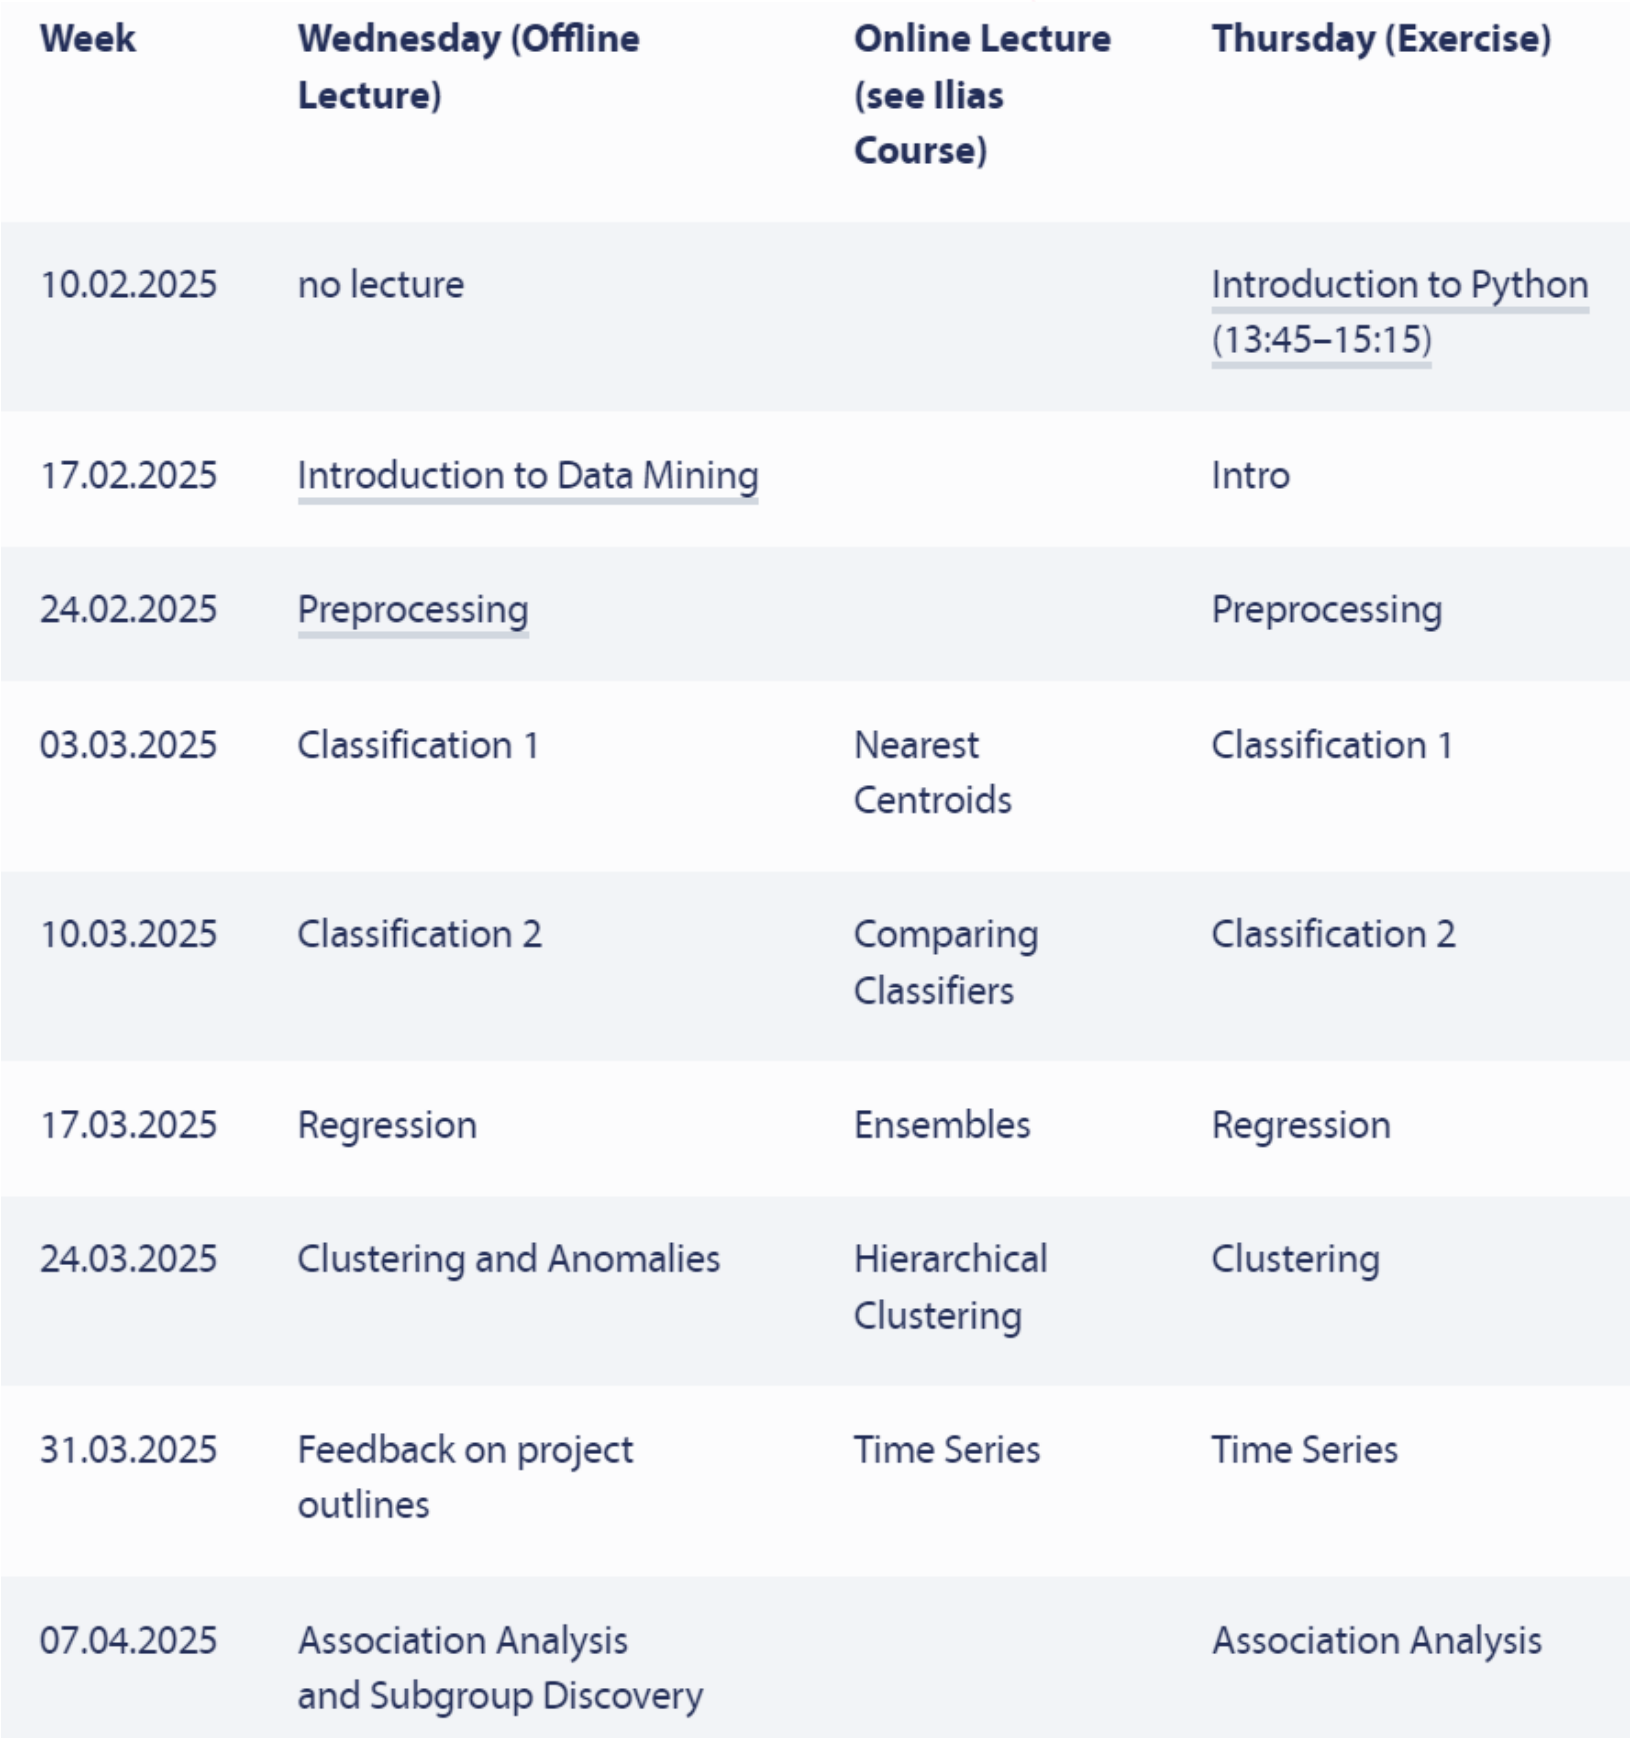
\includegraphics[width=\textwidth,height=4.6cm,keepaspectratio]{images/slide54_online_lecture_screen.png}
      \end{center}
    \end{column}
  \end{columns}
\end{frame}

% Slide 55: Questions
\begin{frame}[plain]
  \begin{center}
    \vspace*{0.8cm}
    {\fontsize{22}{26}\selectfont\color{mannheimblue}\textbf{پرسش و پاسخ}}\\[0.2cm]
    {\fontsize{13}{16}\selectfont\color{subgray}Questions \& Discussion}\\[0.6cm]
    
\includegraphics[height=3.8cm,keepaspectratio]{images/slide55_questions.png}
  \end{center}
\end{frame}

% Slide 56: Literature
\begin{frame}{منابع و مراجع مطالعاتی فصل}{\lr{Literature for this Slideset}}
  \begin{columns}[T]
    \begin{column}{0.65\textwidth}
      \begin{itemize}
        \setlength{\itemsep}{5pt}
        \item \textbf{حل مسائل عملی رگرسیون با پایتون:}
        \begin{latin}
          {\fontsize{8.5}{11}\selectfont
          Aurélien Géron: \textit{Hands-On Machine Learning with Scikit-Learn, Keras, and TensorFlow} (Chapter 4)
          }
        \end{latin}
        \item \textbf{مبانی نظری و تحلیل ریاضی رگرسیون:}
        \begin{latin}
          {\fontsize{8.5}{11}\selectfont
          Gareth James, Daniela Witten, Trevor Hastie, Robert Tibshirani: \textit{An Introduction to Statistical Learning} (Chapters 3, 7, 8)
          }
        \end{latin}
      \end{itemize}
    \end{column}
    \begin{column}{0.32\textwidth}
      \begin{center}
        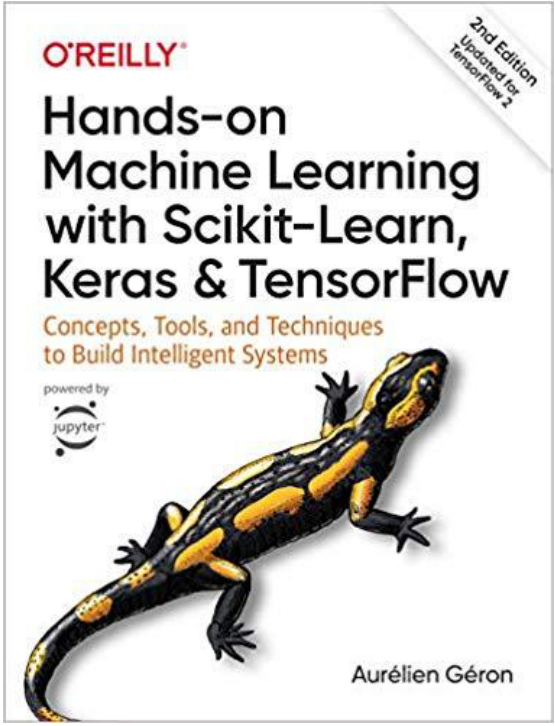
\includegraphics[height=2.3cm,keepaspectratio]{images/slide56_book1.png}\\[0.2cm]
        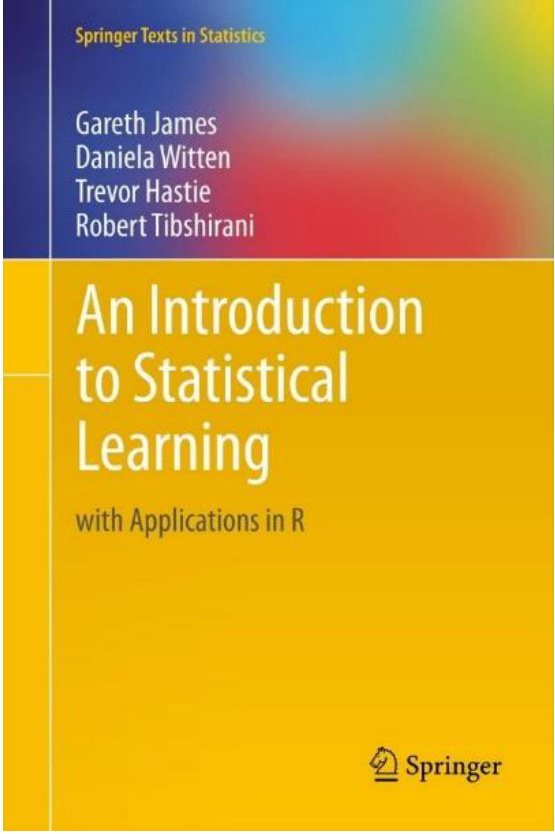
\includegraphics[height=2.3cm,keepaspectratio]{images/slide56_book2.png}
      \end{center}
    \end{column}
  \end{columns}
\end{frame}
